



\section{Cônicas}

\item
 Esboce e determine os elementos principais (focos, vértices, assíntotas, diretriz) das curvas cujas equa\c{c}\~oes s\~ao
\begin{multicols}{02}
  \begin{enumerate}[leftmargin=*]
  \item[a)] $\dfrac{x^2}{25}+\dfrac{y^2}{9}=1$;
  \item[b)] $\dfrac{x^2}{9}+\dfrac{y^2}{25}=1$;
  \item[c)] $\dfrac{x^2}{25}-\dfrac{y^2}{9}=1$;
  \item[d)] $\dfrac{y^2}{9}-\dfrac{x^2}{25}=1$;
  \item[e)] $x=y^2$;
  \item[f)] $y=x^2$;
  \item[g)] $4x^2+9y^2=36$;
  \item[h)] $x^2-y^2+4=0$;
  \end{enumerate}
\end{multicols}
\item Dada a elipse $225x^2 + 289y^2=65025$, esboce seu gráfico e determine:
\begin{multicols}{02}
 \begin{enumerate}[leftmargin=*]
 \item o comprimento do semieixo maior
 \item o comprimento do semieixo menor
 \item as coordenadas dos focos
 \item as coordenadas dos vértices
 \end{enumerate}
 \end{multicols}
\item Determine a equação da elipse de focos $(\pm 3,0)$ e que passa pelo ponto $(0,4)$.
\item Determine a equação da elipse com centro na origem, um foco em $(0,3)$ e eixo maior medindo 10 unidades. 
\item
  Determine uma equação da hipérbole cujas assintotas s\~ao $y=x$ e $y=-x$, sabendo-se que um de seus vértices \'e o ponto $(2, 0)$.
  
 \item Determine o valor de $k$ para que a parábola $y=kx^2$ tenha foco no ponto $(0,3)$. Esboce a parábola encontrada no sistema de coordenadas cartesianas.
  
 \item Determine os pontos em que a reta $x+y=1$ intercepta a parábola $x^2-y=0$.
  
 \item Determine a equação da hipérbole que satisfaz as condições dadas.
  
 \begin{enumerate}[leftmargin=*]
   \item Focos $(0,\pm 4)$ e vértices $(0,\pm 1).$
   \item Focos $(\pm 5, 0)$ e vértices $(\pm 3, 0).$
   \item Vértices $(\pm 3, 0)$ com assíntotas $y=\pm 2x.$
 \end{enumerate}
 \item Ache a equação da hipérbole cujos focos são os vértices da elipse $7x^2+11y^2=77$ e cujos vértices são os focos dessa elipse.
   
\item Determine a equação da circunferência circunscrita ao triângulo de vértices $A(1,4)$, $B(3,-2)$ e $C(7,2).$
 
\item Determine a equação da elipse com focos $(0,\pm 3)$ e eixo maior de comprimento $6\sqrt{3}$. 
  
  
\item Determine a equação da hipérbole de centro $(-2,-1)$, vértice $(-2,11)$ e foco $(-2,14)$.
\item Esboce a curva dada pela equação:
  \begin{multicols}{02}
\begin{enumerate}[leftmargin=*]
   \item $x^2+y^2-2x-6y+6=0$
   \item $2x^2 + y^2 + 16x - 4y +32=0$
   \item $x^2-3y^2+6x + 6y + 3=0$
   \item $y^2-4y-2x+2=0$
   \item $y^2-10y-8x+17=0$
   \item $y^2+8y-2x+22=0$
   \end{enumerate}
\end{multicols}
  \item
 Prove que numa parábola o comprimento da corda que contém o foco e é perpendicular ao eixo \'e duas vezes a dist\^ancia do foco \`a diretriz.
 \item
 Mostre que qualquer que seja o valor de $t$ o ponto
$$(a \cos t, b \sin t )$$
pertence elipse
$$\frac{x^2}{a^2}+\frac{y^2}{b^2}=1.$$
\textit{Observação}: Quando $t$ varia de $0$ a $2\pi$ o ponto $(a \cos t,b \sin t)$ percorre a elipse, a partir do vértice
$A(a, 0)$, uma vez.
$$
\begin{cases}
x=a\cos(t),\\
y=b\sin(t),
\end{cases}
$$
s\~ao equações paramétricas da elipse.
\section{Suplementares} 
\item
 Deduzir uma equação
 \begin{enumerate}[leftmargin=*]
 \item[a)] da elipse cujos focos são,$F_1(-1,-1)$ e $F(1,1)$ e o eixo maior \'e $4\sqrt{2}$.
 \item[b)] da hipérbole cujos focos $F_1(-1,-1)$ e $F(1,1)$ e o eixo \'e $\sqrt{2}$.
 \item[c)] da parábola de foco $F(0,0)$ e diretriz $y=2$.
 \end{enumerate}
  
\item
 Deduza uma equação da parábola com v\'ertice em $V(6,-3)$ e cuja diretriz \'e a reta $3x-5y+1=0$.
 

  
 \item
  Escrever uma equação da elipse cujos focos  s\~ao $F_1(-2,1)$ e $F_2(2,3)$ e o eixo menor mede $4$.
 

\item\label{tangente}
 Demonstre que a reta
$$\frac{x_0x}{a^2}+\frac{y_0y}{b^2}=1,$$
\'e tangente \'a elipse
$$\frac{x^2}{a^2}+\frac{y^2}{b^2}=1,$$
no ponto $P(x_0,y_0)$. [\textit{Dica: Use derivadas. }] 

\item
 Determine o valor de $k$ para que e reta
$$\frac{2x}{9}+\frac{ky}{4}=1,$$
seja tangente à elipse
$$\frac{x^2}{9}+\frac{y^2}{4}=1.$$
 [\textit{Dica: Use o Exercício \ref{tangente}.}] 

\item
  Determine o ponto da elipse 
 $$\frac{x^2}{18}+\frac{y^2}{8}=1$$
mais próximo da reta $2x -3y+ 25 = 0$.
 

\item
  Considere uma semi-elipse e uma semi-reta como mostra a figura abaixo. Se girarmos a semi-reta no sentido
hor\'ario, em torno de $P$, em qual ponto da elipse ela tocar\'a?
\begin{figure}[H]
 \begin{center}
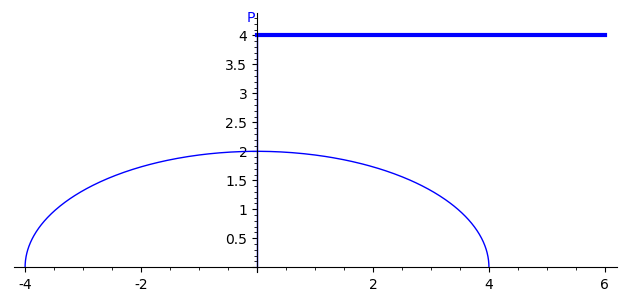
\includegraphics[scale=0.5]{sections/tmp_DSBM_N.png}
\caption{a)}
\end{center}
 \end{figure}
  

 
 \item
 Determine os valores de $m$ para os quais a reta
$$y=\frac{5}{2}x+m$$
\'e tangente a hipérbole
$$\frac{x^2}{9}-\frac{y^2}{36}=1
$$
[\textit{Dica: Use derivadas. }] 
% 
\item
 Seja $P$ o pé da perpendicular baixada do foco $F$ da hipérbole
$$\frac{x^2}{a^2}-\frac{y^2}{b^2}=1$$
a uma das assíntotas. Demonstre que $\overline{PF} = b$ e $\overline{PO} =a$, onde $O$ é a origem do sistema de coordenadas.
 

\item
 Prove que toda parábola cujo eixo \'e paralelo ao eixo $y$ tem uma equação da forma
$$y=ax^2+bx+c.$$
Qual é a forma geral das equações das parábolas cujo eixo é paralelo ao eixo $x$?
 

\item
 Deduzir uma equação da parábola que contém o ponto $(1, 4)$, sabendo-se que seu eixo é paralelo ao eixo $y$ e que seu v\'ertice é o ponto $(2,3)$.
 
% 
\item
 Deduza uma equação da parábola que contém os pontos $(-1,12), (1,2),(2,0)$ 
e tem eixo pararelo ao eixo $y$.
 
% 

 

\item
   \begin{enumerate}[leftmargin=*]
  \item[a)] Prove que a reta $x-2ay_0y+x_0=0$ \'e tangente à parábola $x= ay^2$ no ponto $P(x_0,y_0)$. [\textit{Dica: Use derivadas. }] 
  \item[b)] Mostre que a perpendicular \`a tangente em $P(x_0,y_0)$ \'e bissetriz do \^angulo formado por $PF$ (onde $F$ é o foco da parábola) e a paralela ao eixo da parábola que contém $P(x_0,y_0)$.
  \end{enumerate}
 

% 

 

\item
 Um part\'icula se move de modo que no instante $t$ seu vetor posi\c{c}\~ao \'e
 $$\vec{OP}(t)=(t,4t-t^2).$$
 Determine
  \begin{enumerate}[leftmargin=*]
  \item[a)] uma equa\c{c}\~ao cartesiana da trajet\'oria da particula;
  \item[b)] o instante em que a particula se encontra mais pr\'oxima da reta $y=5$.
  \end{enumerate}

 






























% \item Determine se são verdadeiras ou falsas as seguintes afirmações.
% \begin{enumerate}[leftmargin=*]
% \item  Duas retas paralelas a uma terceira são paralelas.
% \item  Duas retas perpendiculares a uma terceira são paralelas.
% \item  Duas retas paralelas a um plano são paralelas.
% \item  Duas retas perpendiculares a um plano são paralelas.
% \item  Duas retas ou se interceptam ou são paralelas.
% \end{enumerate}

% \item[\textcolor{blue}{44-45}] Obtenha equações paramétricas para a reta que passa pelos pontos
% $P$ e $Q$ e também para o segmento de reta ligando esses pontos.
% \item 
% \begin{enumerate}[leftmargin=*]
%     \item $P(3, -2),\quad Q(5, 1)$
%     \item $P(5, -2, 1),\quad Q(2, 4, 2)$
% \end{enumerate}
% \item 
% \begin{enumerate}[leftmargin=*]
%     \item $P (-1, 3, 5), \quad Q(-1, 3, 2)$
%     \item $P (-1, 3, 5),\quad Q(-1, 3, 2)$
% \end{enumerate}
% \item[\textcolor{blue}{46-50}] Obtenha equações paramétricas da reta que satisfaz as condições dadas.

% \item A reta que passa por $(-5, 2)$ e é paralela a $\vb=2\ib - 3\jb$.
% \item A reta que é tangente ao círculo $x^2 + y^2 = 25$ no ponto $(3,-4)$.
% \item A reta que é tangente à parábola $y = x^2$ no ponto $(-2, 4)$.

% \item A reta que passa por $(-2, 0, 5)$ e é paralela à reta $x = 1 + 2t$, $y = 4 - t$, $z = 6 + 2t$.
% \item A reta que passa pela origem e é paralela à reta $x = t$, $y = -1+ t$, $z = 2$.

% \item Em que ponto a reta $x = 1 + 3t$, $y = 2 - t$ intersecta
% \begin{enumerate}[leftmargin=*]
% \begin{multicols}{3}
%     \item o eixo $x$
%     \item o eixo $y$
%     \item a parábola $y=x^2$?
%     \end{multicols}
% \end{enumerate}
% \item Encontre a intersecção da reta $x = -2$, $y = 4 + 2t$, $z = -3 + t$ com os planos $xy$ e $xz$.

% \item Determine a projeção ortogonal do ponto $P(2,-1, 3)$ sobre a reta $x=3t,\, y=-7+5t,\, z=2+2t$.


% \item Considere o triângulo de vértices $A(1,0,-2)$, $B(2,-1,-6)$ e $(-4, 5, 2)$. Determine as equações paramétricas da reta suporte da mediana relativa ao lado $BC$.

% \item Considere o triângulo de vértices  $A(3,3,3)$ , $B(0, 1, 3)$ e $C(6, 15, -3)$ . Determine as equações paramétricas da reta suporte da altura relativa ao lado $BC$.

% \item[\textcolor{blue}{56-60}] Determine a posição relativa das retas $r_1$ e $r_2$.

% \item $r_1: x = 2 + t,\, y = 2 + 3t,\, z = 3 + t$ \\ $r_2: x = 2 + s, \,y = 3 + 4s,\, z = 4 + 2s$

% \item $r_1 : x = 1 + 7t, \,y = 3 + t, \,z = 5 - 3t$\\
% $r_2 : x = 4 - s, \,y = 6, \,z = 7 + 2s$    

% \item $r_1 : x = 2 -t, \,y = 3 + 2t, \,z = 1 + t$\\
% $r_2 : x = 5 - 2s, \,y = 2+4s, \,z = 1 + 2s$ 

% \item $r_1 : x = 2 +t, \,y = -3 -t, \,z = t$\\
% $r_2 : x = \frac{1}{2}(3s + 1), \,y = s-1, \,z = \frac{1}{3}s$   
% \item $r_1 : x = 2 +t, \,y = 4 - 2t, \,z = 1 + 3t$\\
% $r_2 : x = -1 + 4s, \,y = 3-s, \,z = 2 + 2s$ 

% \item Determine a distância do ponto $A(-2,1,2)$ à reta determinada pelos pontos $P(1,2,1)$ e $Q(0,-1,3)$.
% \item Determine a medida da projeção ortogonal de $\vb=\ib + 2\jb + \kb$ sobre a reta $x=1-2t$,$y=t$, $z=-1-2t$.
% \section{Planos}
% \item Determine se são verdadeiras ou falsas as seguintes afirmações.
% \begin{enumerate}[leftmargin=*]
%     \item  Dois planos paralelos a um terceiro são paralelos.
%     \item  Dois planos perpendiculares a um terceiro são paralelos.
%     \item  Dois planos paralelos a uma reta são paralelos.
%     \item  Dois planos perpendiculares a uma reta são paralelos.
%     \item  Dois planos ou se interceptam ou são paralelos.
%     \item  Um plano e uma reta ou se interceptam ou são paralelos.
% \end{enumerate}


% \item Determine uma equação do plano nos casos citados.

% \begin{enumerate}[leftmargin=*]
% \item passa pelo ponto $P(2, 6, 1)$ e tem $\mathbf{n}= \lan 1, 4, 2\ran$ como um vetor normal. 

% \item passa pelo ponto $P(-1, -1, 2)$ e tem $\mathbf{n}= = \lan -1, 7, 6\ran$ como um vetor normal. 

% \item que passa pelos pontos $A(-2, 1, 1)$, $B(0, 2, 3)$ e $C(1, 0, -1)$.

% \end{enumerate}
% \item Determine uma equação do plano nos seguintes casos:
% \begin{enumerate}[leftmargin=*]
%     \item paralelo ao plano $2x-3y-z+5=0$ e que passa pelo ponto $P(4,-1,2)$.
%     \item perpendicular à reta $x=1-3t$, $y=5+2t$, $z=-t$ e que passa pelo ponto $P(4,-1,2)$.
%     \item determinado pelas retas  $x=1+2t$, $y=4t$, $z=-1+6t$ e  $x=s$, $y=1+2s$, $z=-2+3s$
%     \item perpendicular ao eixo $y$ e que passa pelo ponto $P(-1,0,2)$.
%     \item determinado pelo ponto $P(3,-1,2)$ e pela reta $x=t$,$y=2-t$, $z=3+2t$.
% \end{enumerate}


% \item Determine uma equação do plano determinado pelo ponto $P(3,-2,-1)$ e pela reta de intersecção dos planos
%             $x+2y+z-1=0$ e   $2x+y-z+7=0$.
% \item  Determine uma equação do plano determinado pelo ponto $P(1,2,1)$ e pela reta de intersecção dos planos $x-2y+z-3=0$ e $x=0$.

% \item Determine uma equação do plano que contém o ponto $P(2, 0, 3)$ e a reta $x = -1 + t$, $y = t$, $z = -4 + 2t$.

% \item[\textcolor{blue}{69-70}] Obtenha equações paramétricas da reta de interseção dos planos dados.

% \item $\pi_1: -2x + 3y + 7z + 2 = 0$\\
% $\pi_2: x + 2y - 3z + 5 = 0$
% \item $\pi_1: 3x - 5y + 2z = 0$\\
% $\pi_2: z=0$
% \item Determine a distância entre o ponto $P(1, -2, 3)$ e o plano $2x - 2y + z = 4$.
% \item Determine a distância entre os planos paralelos $-2x + y + z = 0$ e $6x - 3y - 3z - 5 = 0$.

% \section{Problemas Suplementares II}
% \item Mostre que a distância entre os planos paralelos 
% \begin{align*}
%     \pi_1: ax+by+cz + d_1=0\\
%     \pi_2: ax+by+cz + d_2=0
% \end{align*}
% é 
% \begin{align*}
%     D=\dfrac{|d_1-d_2|}{\sqrt{a^2+b^2+ c^2}}
% \end{align*}
% \item Se $a$, $b$ e $c$ não são todos nulos, mostre que a equação $ax + by + cz+ d = 0$ representa um plano e $\lan a, b, c\ran$ é o vetor normal ao plano.

% \item Determine uma equação do plano cujos pontos são equidistantes de $P_1(2, -1, 1)$ e $P_2(3, 1, 5)$.

% \item Determine a equação paramétrica da $r$ que passa pelo ponto $P(1,2,0)$ e é paralela à reta de intersecção dos planos $2x-y-z+1=0$ e $x+3y+2z-4=0$
% \item Suponha que $\vb_1$ e $\vb_2$ sejam vetores com $\|\vb_1\| = 2$, $\| \vb_2\| = 3$ e $\vb_1 \cdot \vb_2 = 5$. Seja $\vb_3 = \mathrm{proj}_{\vb_1} \vb_2$ , $\vb_4 = \mathrm{proj}_{\vb_2} \vb_3$, $\vb_5 = \mathrm{proj}_{\vb_3} \vb_4$  e assim por diante. Calcule $\sum_{n=1}^{\infty}\|\vb_n \|$.
% \item Determine uma equação da esfera com centro $(2, 1, -3)$ que é tangente ao plano $x - 3y + 2z = 4$.

% \item Determine a distância entre as retas reversas 
% \begin{align*}
%     r_1: & x = 1 + 7t, \, y = 3 + t, \, z = 5 - 3t\\
%     r_2: & x = 4 - s,\, y = 6,\, z = 7 + 2s
% \end{align*}
% $$.$$